\chapter{Prototype Design}
\label{chap:prototype}

\section{Overview}

Throughout the course of this dissertation work, the Rapidly Reconfigurable Research Cockpit (R3C) prototype underwent many changes and improvements to the technology used.
Our underlying motivation and goals of the technical approach of the prototype remained as described in the previous chapter, but as technology evolved and our experience and feedback grew, a number of improvements and revisions were developed.
In this chapter, three major versions of the prototype are outlined here, and the evolution of the technical approach is described.
The first prototype was not used in a formal experiment, but two versions based on the second prototype were used for the first two research studies (Chapter \ref{chap:pointing} and \ref{chap:ph_exp}).
The final prototype was used in the third experiment (Chapter \ref{chap:de_exp}).

\section{Requirements}

The motivations described in the previous chapter led to a few high level requirements for the Rapidly Reconfigurable Research Cockpit (R3C) prototype.
These requirements guided the development of the prototypes, based on the technology available.

\begin{description}
    \item [Rapid prototyping of physical mockup.]
        Based on the motivation of enabling more rapid redesign iterations, the R3C system should allow for rapid changes in the physical world without needed to reconfigure the software heavily, or reconfigure any hardware for interaction.
    \item [Minimal setup and calibration.]
        Our motivation to use this system in early design stages means that we require it be able to be used ``on top'' of existing mockup systems.
        One consequence of this means that as much as possible, the hardware used must be easy to set up and able to use in constrained spaces.
        This eliminates some of the high-end head mounted displays that use complicated head tracker systems requiring precise calibration.
        Additionally, this eliminates many of the past approaches to hand tracking which use multiple cameras precisely calibrated, or magnetic sensors in a well-defined magnetic field.
        The minimal setup also leads to the need for hand tracking, as the recognition of the user input must be done without outfitting the mockup with working input actuators (i.e.\ buttons).
    \item [Immersive head mounted display.]
        The need for an immersive HMD with a large field of view is based on the need to use the system as a design evaluation tool.
        Without the ability to place visuals on the screens or create out-the-window views, design evaluations may not be as useful.
        Current augmented reality or mixed reality goggles do not provide the same level of immersion that a fully virtual display provides.
    \item [Unobtrusive hand tracking.]
        For a realistic design evaluation, it is important that the hand tracker does not modify the users behavior.
        Many hand trackers use a glove or other marker worn on the hand to provide the tracking ability.
        Newer optical-based hand trackers allow this requirement to be fulfilled.
\end{description}

\section{Prototype Development}

\subsection{First Prototype}

The first prototype was the proof of concept of the system, and before it could be used for a formal research study, it was quickly outdated with new technology and software updates.
However, many informal feedback sessions did help highlight the usability and technical issues that led to the next prototype.
The software developed during this prototype also provided a significant base for the software used throughout all the prototypes.
The hardware used for this prototype was the first generation Oculus Rift Development Kit and the first generation of software for the LeapMotion hand tracker.

\subsubsection{Rendering Engine}

We are using a NASA developed rendering engine named EDGE to provide the visuals for the virtual scene rendered in the head-mounted display (HMD).
EDGE is highly customizable and extendable through C/C++ plugins, Tcl scripts, or networking functions.
Many of the integrations described in the prototypes were created as EDGE plugins.
This rendering engine was used in all subsequent prototypes and research studies.

\subsubsection{Virtual Reality Headset}

The head-mounted display (HMD) we used for the first prototype was an Oculus Rift Development Kit (Figure \ref{fig:proto_oculus}).
The lightweight headset provides an immersive virtual reality experience by combining a wide field-of-view scene with accurate head tracking, giving a stable virtual world.
The small display (cell phone sized) is viewed through a single set of lenses, and the barrel distortion of the lens is corrected for in the rendering engine by a pincushion distortion of the rendered scene.
The orientation of the head is tracked using internal sensors (accelerometer, gyroscope and magnetometer).
The software developer’s kit (SDK) exposes the head orientation and provides the appropriate distortion for a rendered scene (which is done for each eye), and this was developed into an EDGE plugin.
The first generation Oculus Rift Development Kit has a 1280x800 LCD screen (with 640x800 for each eye) with a refresh rate of 60Hz.
The field of view is approximately $110^{\circ}$.

\begin{figure}
    \centering
    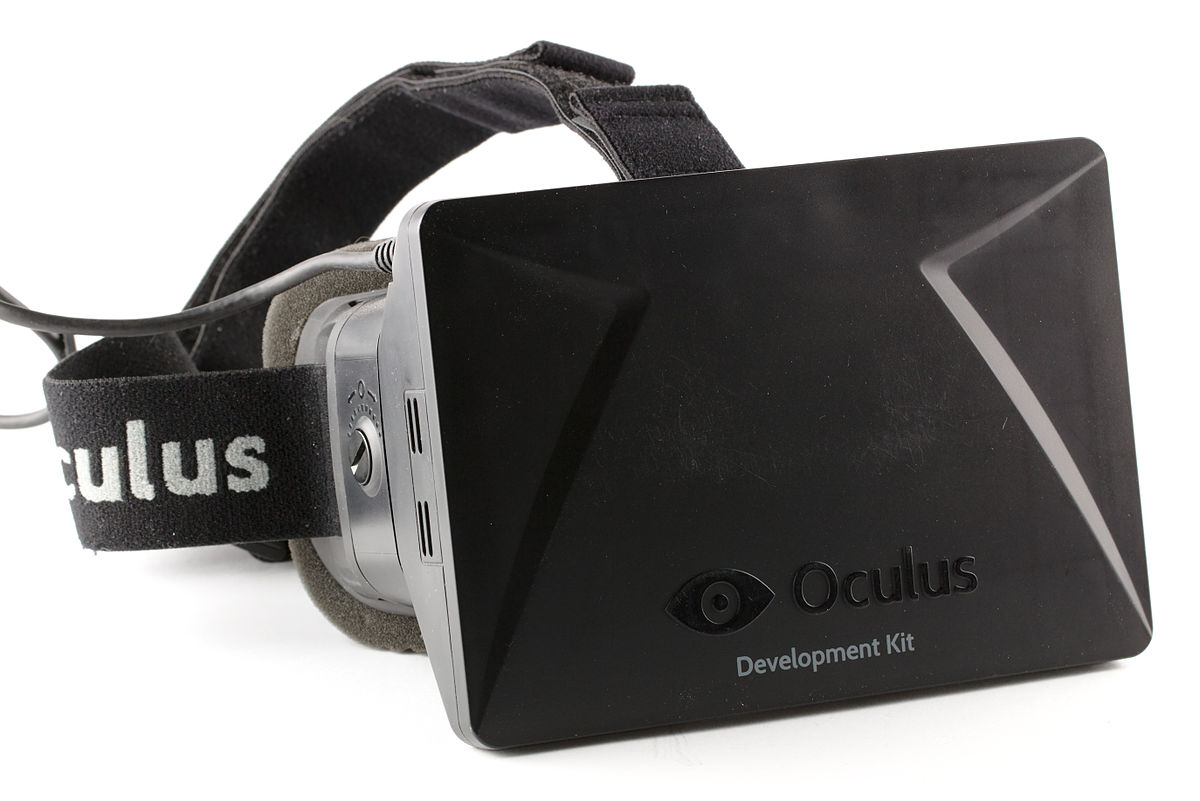
\includegraphics[width=3in]{proto_dk1.jpg}
    \caption{The original Oculus Rift Development Kit.}
    \label{fig:proto_oculus}
\end{figure}

\subsubsection{3D Printed Instruments}

A central tenant of our technical approach is to use physical, geometrically accurate instrument shapes that provide no functionality (i.e.\ no screens, no working buttons, etc.).
This is due to the motivation of being able to be used in an early design stage mockup.
In order to achieve this we have produced 3D-printed ``instruments'' that can be easily rearranged on a panel mount (pegboard).
Since the devices are rapidly prototyped, they can be redesigned in a much smaller time frame than typical simulator instruments.
By using the geometrically accurate instruments at the correct cockpit locations, the user is provided with accurate tactile and proprioceptive feedback without the need for entering the challenging field of virtual haptic feedback.

To use an instrument in the R3C system, it needs two versions of the 3D model.
The first is the version for the rendering engine, which requires textures and possible work to reduce the number of polygons so that rendering is not slowed down by the model.
The second model is for the 3D printing, which depending on the 3D printer used, will often require small changes to allow for a successful print.
Both of these require a surface mesh model.
Often, the original version exists as a CAD (Computer-Aided Design) model which typically does not describe the surface mesh directly but the geometric models that define the part.
The difficulty of the conversion from CAD to 3D model mesh can depend on the model, and the requirements of the rendering engine.

For this initial prototype, a demo instrument was developed based on a large multi-function display with edge keys.
The instrument model as viewed in the rendering engine is shown in Figure \ref{fig:proto_mfd_render}.
The 3D-printed version is shown pictured in Figure \ref{fig:proto_mfd_print}.
Notice that since it is only used for the tactile feel, it can have a plain aesthetic.
It was also printed in segments due to the limitations of the printer used.
The instrument mounted on a panel and being used is shown in Figure \ref{fig:proto_first_panel}.
This instrument provided a base for the demos, though it the specific design did not end up being used in a research study.
The workflow learned to create this demo instrument was also used for future instruments utilized in the research studies.

\begin{figure}
    \centering
    \begin{subfigure}[t]{0.32\linewidth}
        \centering
        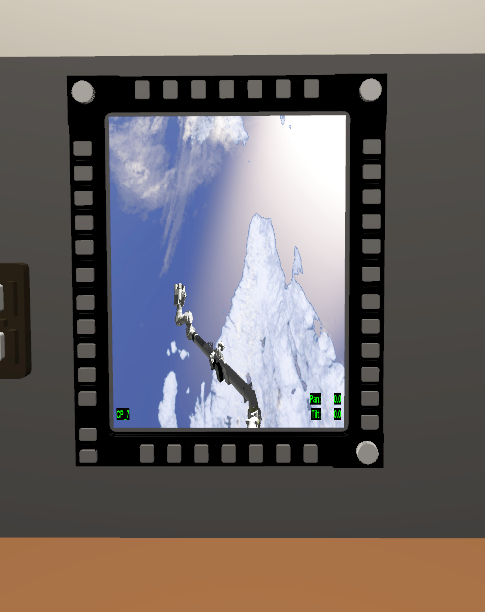
\includegraphics[width=\linewidth]{proto_mfd_render.jpg}
        \caption{The demo multifunction display instrument rendered in the virtual world.}
        \label{fig:proto_mfd_render}
    \end{subfigure}
    \begin{subfigure}[t]{0.32\linewidth}
        \centering
        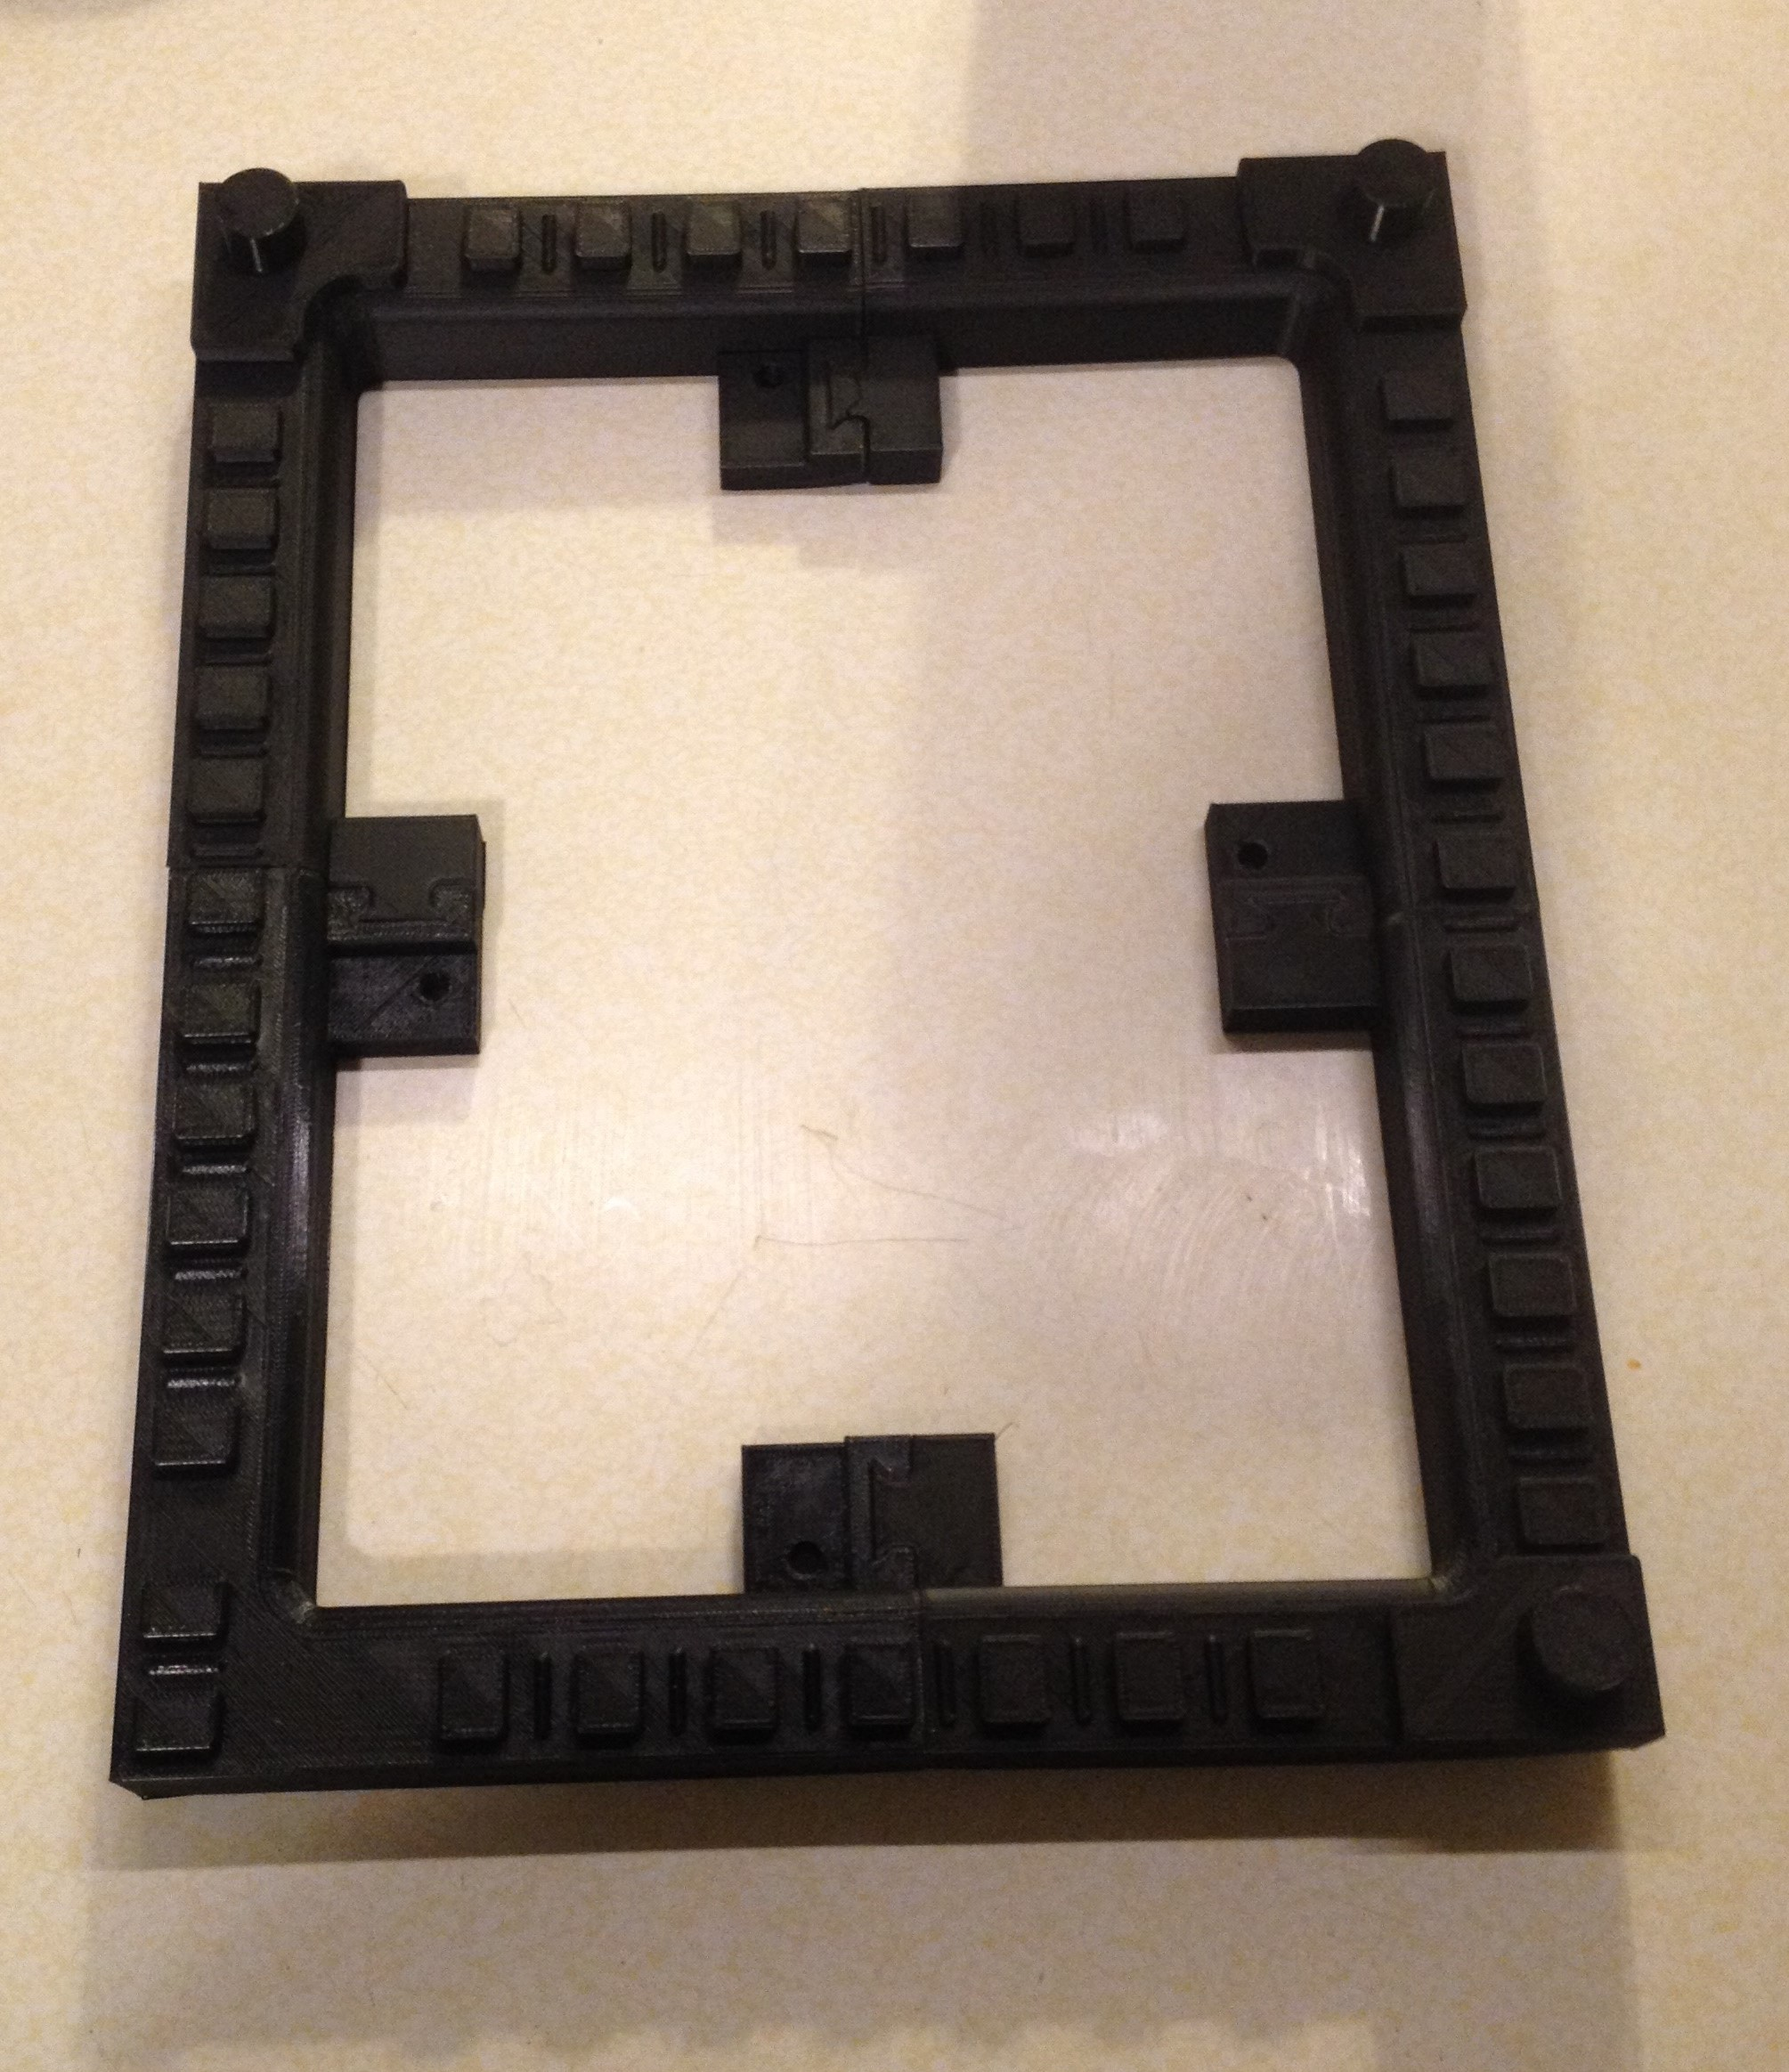
\includegraphics[width=\linewidth]{proto_mfd_print.jpg}
        \caption{The 3D printed version of the demo multifunction display instrument.}
        \label{fig:proto_mfd_print}
    \end{subfigure}
    \begin{subfigure}[t]{0.32\linewidth}
        \centering
        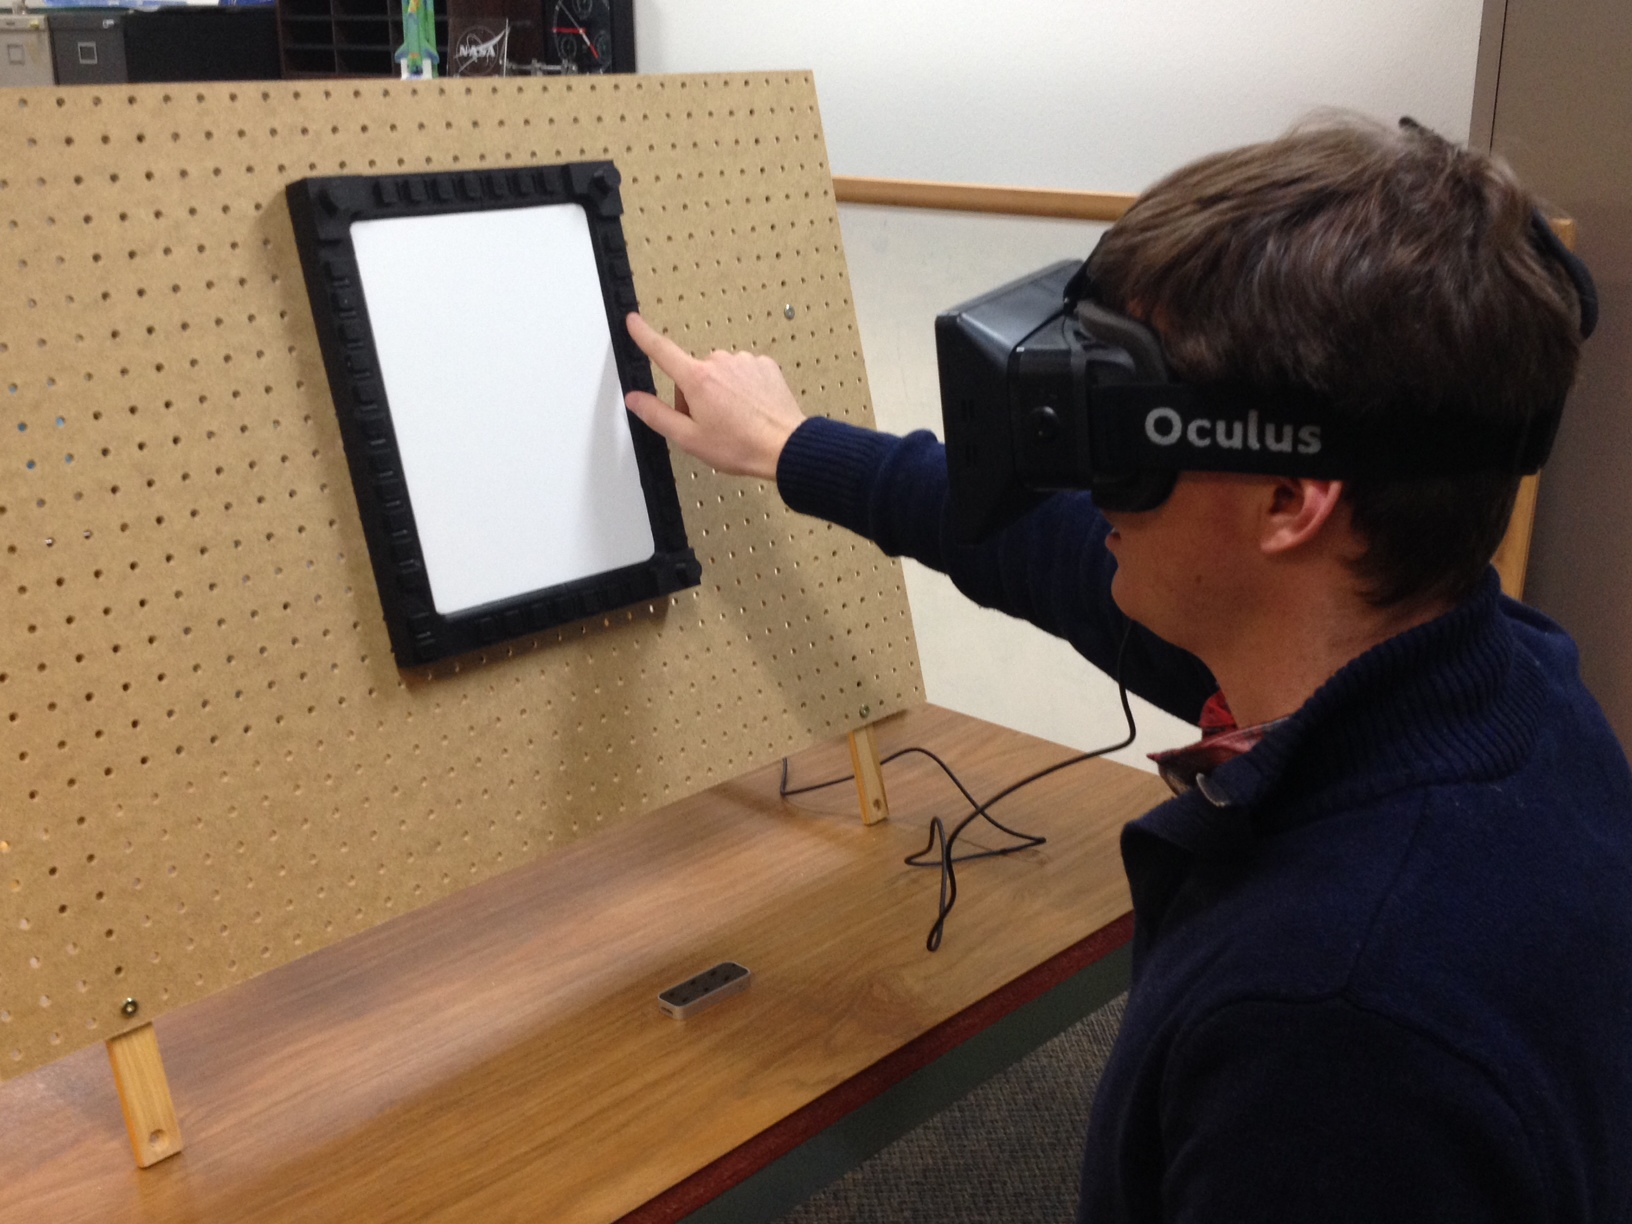
\includegraphics[width=\linewidth]{proto_first_panel.jpg}
        \caption{The demo multifunction display instrument mounted on a panel.}
        \label{fig:proto_first_panel}
    \end{subfigure}
\end{figure}


\subsubsection{Hand Tracking}

The LeapMotion hand tracker was selected as it provided an unobtrusive method for hand tracking.
The device itself is small (3 in x 1.2 in x 0.5 in), allowing it to be used in constrained environments (pictured in Figure \ref{fig:proto_leap_device}).
It uses two infrared cameras as the source of its proprietary tracking algorithm, and requires no gloves to be worn by the user.
The tracking volume extends about 2 feet above the controller, and about 2 feet about the center on the other two axes.
This large field of view is shown in Figure \ref{fig:proto_leap_fov} and can easily cover the working area of a cockpit panel.
The original version of the software, used in this prototype, provided information on the location and orientation of each fingertip.
It also gave the position and orientation of the palm, but did not provide any details on the joints or which finger of the hand the fingertip belonged to.
The tracking rate is approximately 120Hz, with an advertised latency of milliseconds.

\begin{figure}
    \centering
    \begin{subfigure}[t]{0.49\linewidth}
        \centering
        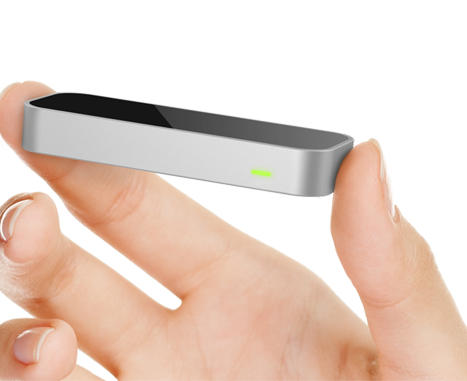
\includegraphics[width=\linewidth]{leapmotion.png}
        \caption{LeapMotion device.}
        \label{fig:proto_leap_device}
    \end{subfigure}
    \begin{subfigure}[t]{0.49\linewidth}
        \centering
        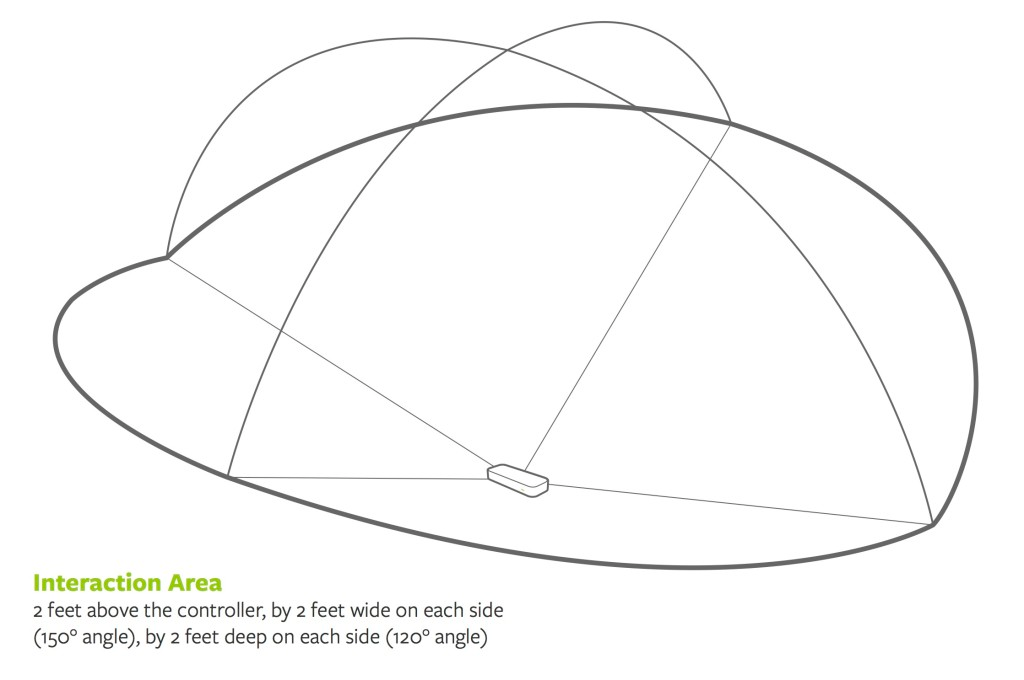
\includegraphics[width=\linewidth]{leapmotion_fov.png}
        \caption{LeapMotion field of view.}
        \label{fig:proto_leap_fov}
    \end{subfigure}
    \caption{The LeapMotion device and field of view. Images by LeapMotion.}
    \label{fig:proto_leap}
\end{figure}

\subsubsection{Button Input Recognition}
\label{sec:proto_button_input}

As part of the motivation and requirements of our approach, the hand tracker data needs to be used to determine when a user is pushing a button.
The goal is to be able to use this system on top of a non-functioning mockup, thus all interactivity must be performed with the hand tracker.
With a working hand tracking system, the next step was to develop a method to determine when users were pushing a button.
The button recognition system was developed within the EDGE engine independent to the hand tracker, so that future prototypes could use a different hand tracker if a new device were released.

The button detection algorithm is a simple collision detection model.
A rectangular box is defined that extends outside the button, including a tolerance zone to account for misalignment and poor tracking.
When a fingertip enters and stays in the box for approximately 150ms\footnote{This time is configurable and was often tweaked for each experiment.} then a button event is triggered.
The purpose of the delay is to account for false positives when a user might accidentally enter the box without intention to press the button.
The advantage to using the optical tracking to determine when a user has selected a button is that it has the potential to significantly reduce the complexity of the system.
If the user interactions with the panel can be determined solely by tracking his/her hands from the external sensor, then the cockpit panel needs only to provide physical feedback, and does not require any wiring.

\subsubsection{Challenges}

The hand tracking caused two issues with the use of the prototype.
The first was simply that the reliability of the tracking caused many instances of dropped tracking, causing fingers to disappear unexpectedly.
The second was the conversion between hand tracker coordinates and instrument coordinates.
The registration between the virtual and physical worlds was difficult to get right with this configuration.
Even with precise alignment of the hand tracker, the fingertip positions did not always align properly with the buttons in the virtual world when a subject had their finger on and felt a physical button.
Since the hand tracking was not very reliable, many users would almost completely ignore its input and find the buttons by proprioception and tactile feedback.
This then led to confusion as the button would not register a button press but the strong tactile feedback meant they would not leave the physical button to hunt for the virtual button location.

Another challenging portion of the registration was that since the Oculus Rift did not have head positioning, the head position would have to be set manually.
Depending on the actual position of the user, the panel would not appear with the correct scale and at the correct distance in the virtual world.
This caused users to initially reach too short or too far for the panel, or decreased the realism as the panel seemed too small or large compared to the real world object.
Since the head tracking sensors were all internal to the headset, it also experienced drift after a few minutes.
Most noticeable in the yaw, it would cause the panel to become misaligned and require a manual reset to realign.

\subsection{Second Prototype}

A number of improvements were made in the second generation of the prototype.
Due to software upgrades, the hand tracking became more robust and provided more complete information about the entire hand position.
The visuals were upgraded to the second Development Kit of the Oculus Rift, which provided improved visual resolution but more importantly an external head tracker (camera) which enabled head movement and virtually eliminated drift of the internal sensors.
A major focus of this version of the development work for this prototype was to improve reliability and registration.
The reliability was partially improved with the new hand tracking software, but other countermeasures developed are described as well.
Registration, which refers to the alignment between the physical world and the virtual world, was improved with the use of a new calibration mechanism described in this section.

\begin{figure}
    \centering
    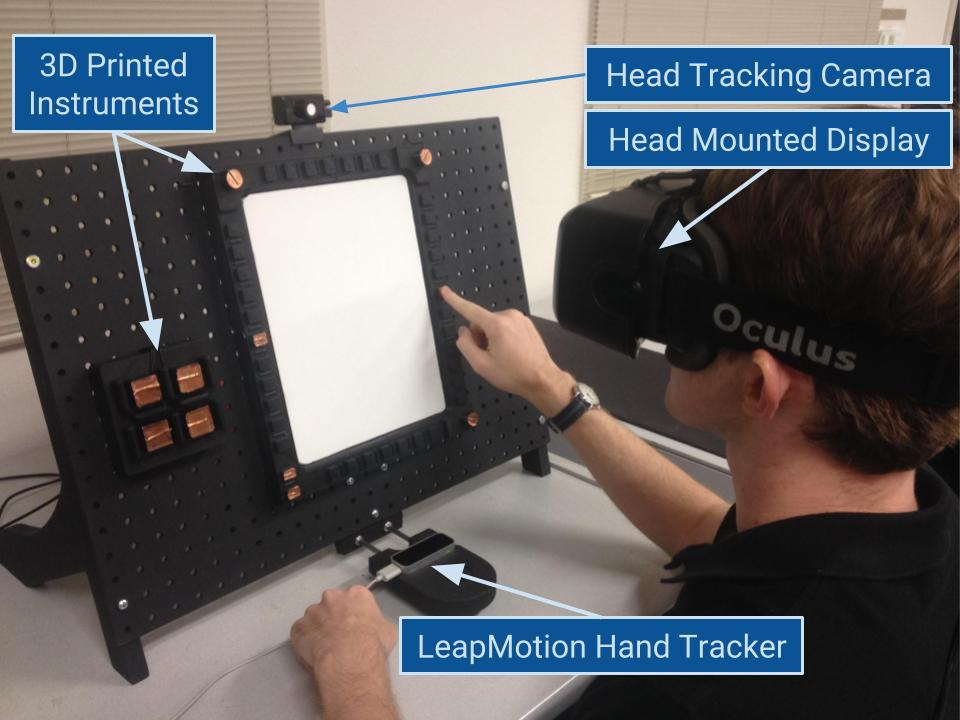
\includegraphics[width=\linewidth]{r3c_callout.jpg}
    \caption{A version of the second prototype with major components noted.}
    \label{fig:r3c_callout}
\end{figure}

\subsubsection{Virtual Reality Headset}

The head tracking provided in the newest development kit version gives a significant improvement over the original Oculus Rift in the registration between the real world and the virtual world.
This allowed the user to lean and gain additional perspective on the virtual world that was not possible with the first version.
The position and orientation is reported relative to the tracking camera which is placed facing the user.
For our application, with a well known location of the camera relative to the panel, the head position can be placed in the virtual world at the exact location of the user's actual head position.
Unlike with the first version, the virtual components are now always rendered at the correct distance and with proper scale.
The head-tracking camera is shown mounted on the instrument panel in Figure \ref{fig:r3c_callout}.


\subsubsection{Hand Tracking}

The upgrade to the hand tracking software provided two features that were integrated.
The first was an improvement in the fidelity of the tracking, including full information on the joints of the hand.
The second was the introduction of a ``head mounted'' mode, which allowed for tracking to be optimized for looking down at a hand.

The tracking upgrade adds the location and orientation of the entire hand at a skeletal level.
This means all the joints are tracked and the bones between them.
The upgraded view is shown in Figure \ref{fig:proto_skeleton}.
This provided a more immersive feeling than the floating fingers of the original prototype.

\begin{figure}
    \centering
    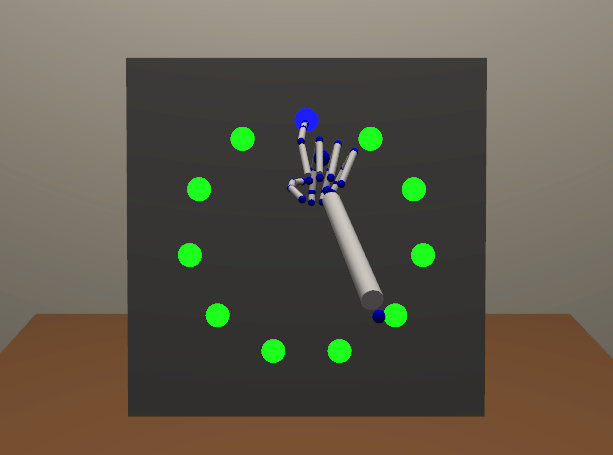
\includegraphics[width=\linewidth]{leap_skeleton.png}
    \caption{The complete hand tracking of the LeapMotion v2 software.}
    \label{fig:proto_skeleton}
\end{figure}

At the same time of the tracking upgrade, a ``VR Mode'' was introduced to the LeapMotion software to provide hand tracking in a virtual environment by way of mounting it on the head-mounted display itself.
Upon initial testing of this feature, two observations were made.
The tracking was much improved when the tracker was looking down at the hands, seemingly providing more robust and reliable tracking data.
However, using it mounted to the head-mounted display caused a larger disconnect between the real world and physical world.
The registration between the hand tracker and the location of the instruments relies on a known, rigid connection.
When the tracker was mounted on the head-mounted display, the transformation between LeapMotion coordinates and panel coordinates relied on knowing the location of the head.
Although this information could be obtained from the newer model HMD which included head tracking, it was simply not precise or stable enough to use as the base for the hand tracking coordinates.
For example, if a hand was placed resting on the panel and kept still, the virtual hand would appear to move relative to the virtual panel if the head were moved at even a moderate pace.
The additional latency introduced by relying on the head tracking sensors simply would not keep accurate registration.
This led us to develop a mount that would hold the LeapMotion upside down over the panel and instruments (Figure \ref{fig:proto_leap_mount}).
The software could still be configured to the ``VR Mode'', optimizing for face-down tracking, but with a rigid mount.
This provided the best of both worlds: reliability of the face-down tracking with a stable transformation between the tracker coordinates and the panel coordinates.

\begin{figure}
    \centering
    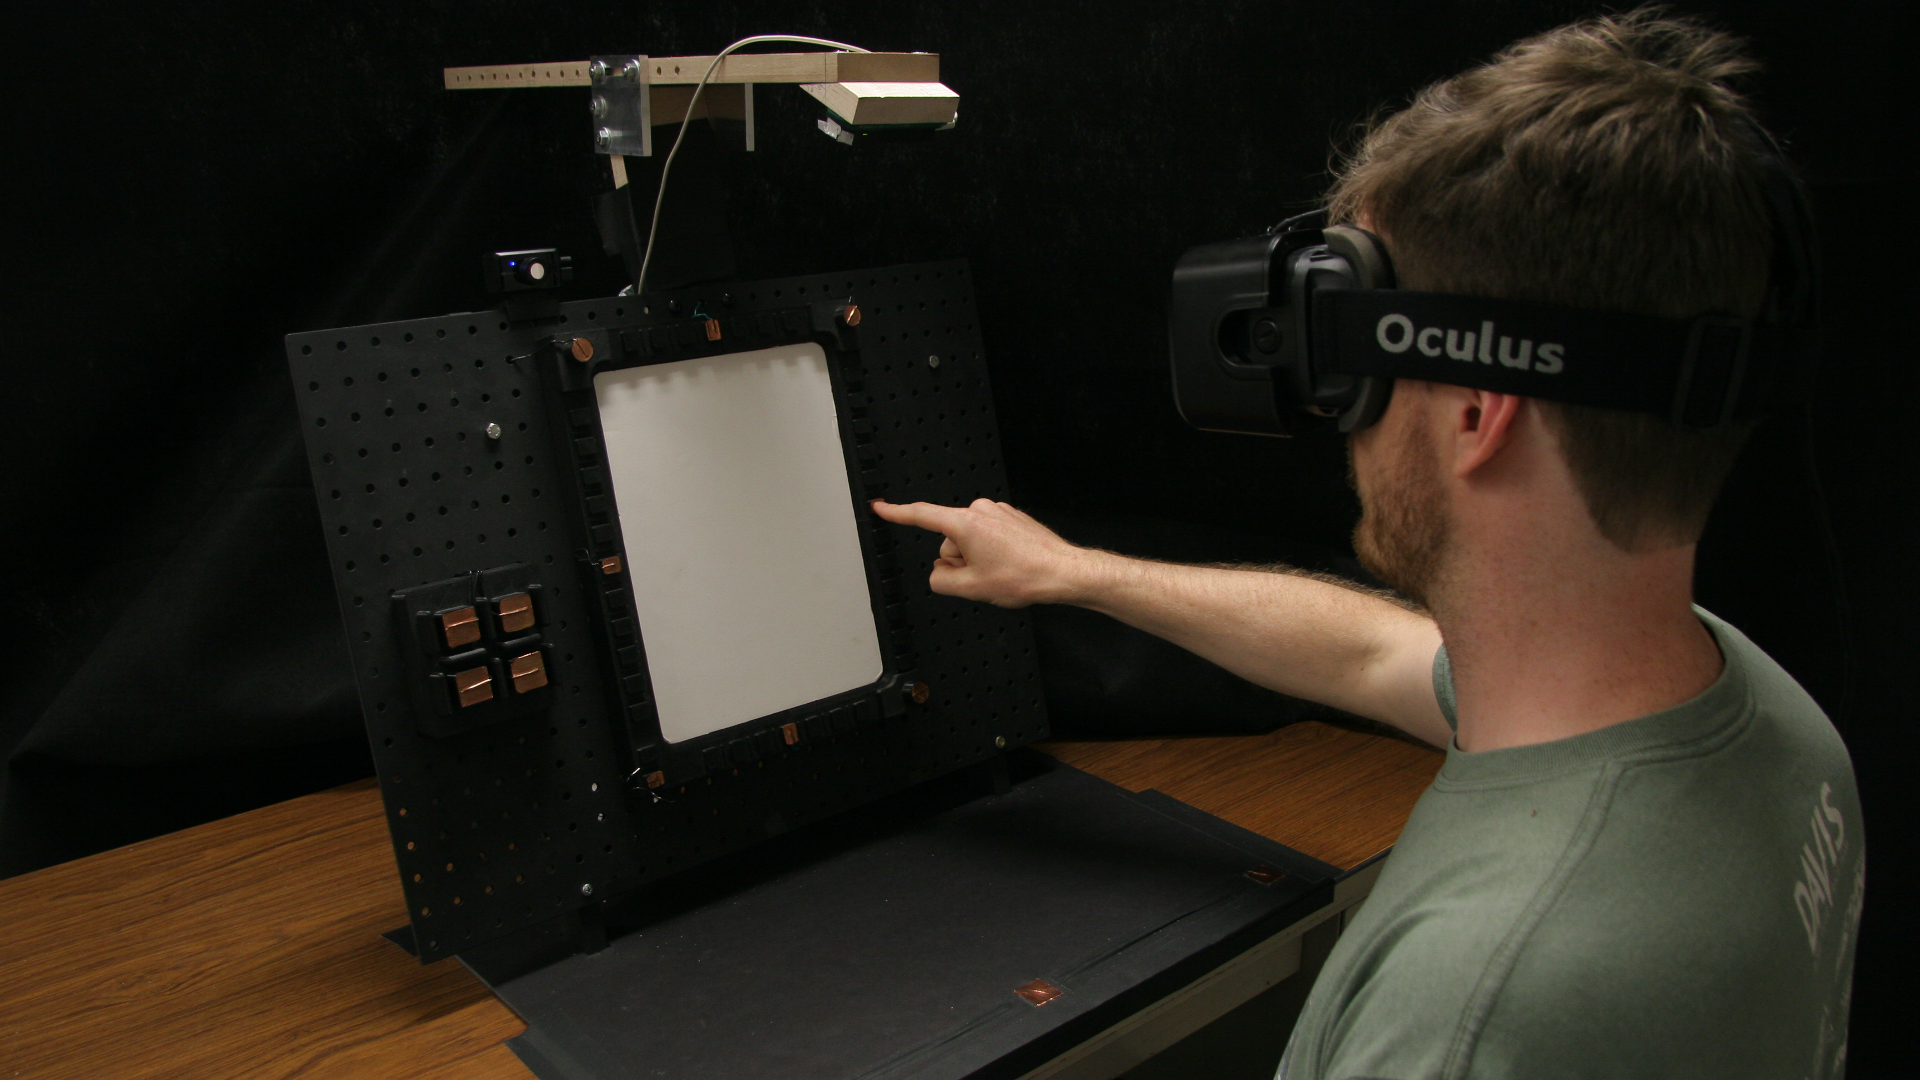
\includegraphics[width=\linewidth]{leap_mount.jpg}
    \caption{The LeapMotion mount, holding the sensor above the panel and looking down.}
    \label{fig:proto_leap_mount}
\end{figure}

\subsubsection{Button Recognition Countermeasures}

%onboarding
Two countermeasures were introduced in this prototype that aided new users in learning the button recognition algorithms of the hand tracker.
A simple visual indication was added when a user entered the zone in front of the button.
This was typically implemented with the button itself being highlighted or changing color.
With this crucial feedback, new users were able to learn the tolerances of the button zone and understand when the button was going to be `pressed'.
For experienced users, the feedback provided confirmation that they were in the zone and were not waiting for it to register incorrectly.
The second countermeasure was the addition of an aural feedback upon the button press being registered.
A simple ``click'' noise was played when the button press event occurred, confirming the button press to the user on a quicker cognitive channel than processing if the expected change on the instrument occurred.
At the same time, the button highlight was restored to the original non-highlighted state, providing feedback in both visual and aural channels.
These countermeasures were observed as being very helpful to new users, and were included in all of the research studies.

\subsubsection{Capacitive Touch Sensors}
\label{sec:proto_cap_touch}

In order to be able to activate the buttons reliably when the hand tracking was degraded or dropped out, it was decided to investigate the use of capacitive touch sensors.
The capacitive touch sensors were initially developed as a countermeasure to the problems encountered with the hand tracking from the original prototype.
As the hand tracking became more robust with the new software from the manufacturer, the countermeasure was not as important, but the sensors played a new role in the prototype: validating the accuracy, and providing calibration for the hand tracker.

With the goal of minimal setup, the original capacitive touch sensors were developed with copper tape electrodes placed on the top of the 3D printed instrument buttons.
These electrodes are shown on the demo multifunction instrument in Figure \ref{fig:copper_pads}.
A Freescale MPR121 capacitive touch sensor was used to read the electrodes and communicate with an Arduino which sent touch events over a serial communication line to the computer.
These serial events were read by the rendering engine to trigger events when a copper pad was touched.
These simple, single electrode per button sensors provided a reliable method for determining when the user had actually touched a button.
The main use of these sensors evolved to be for the calibration mechanism described in the next section.
However, as the registration improved, a research question was developed around how accurate the user could be on the physical device while immersed visually in the virtual world.
This led to the development of a second generation of capacitive touch buttons, used in the Pointing Experiment (Chapter \ref{chap:pointing}).

\begin{figure}
    \centering
    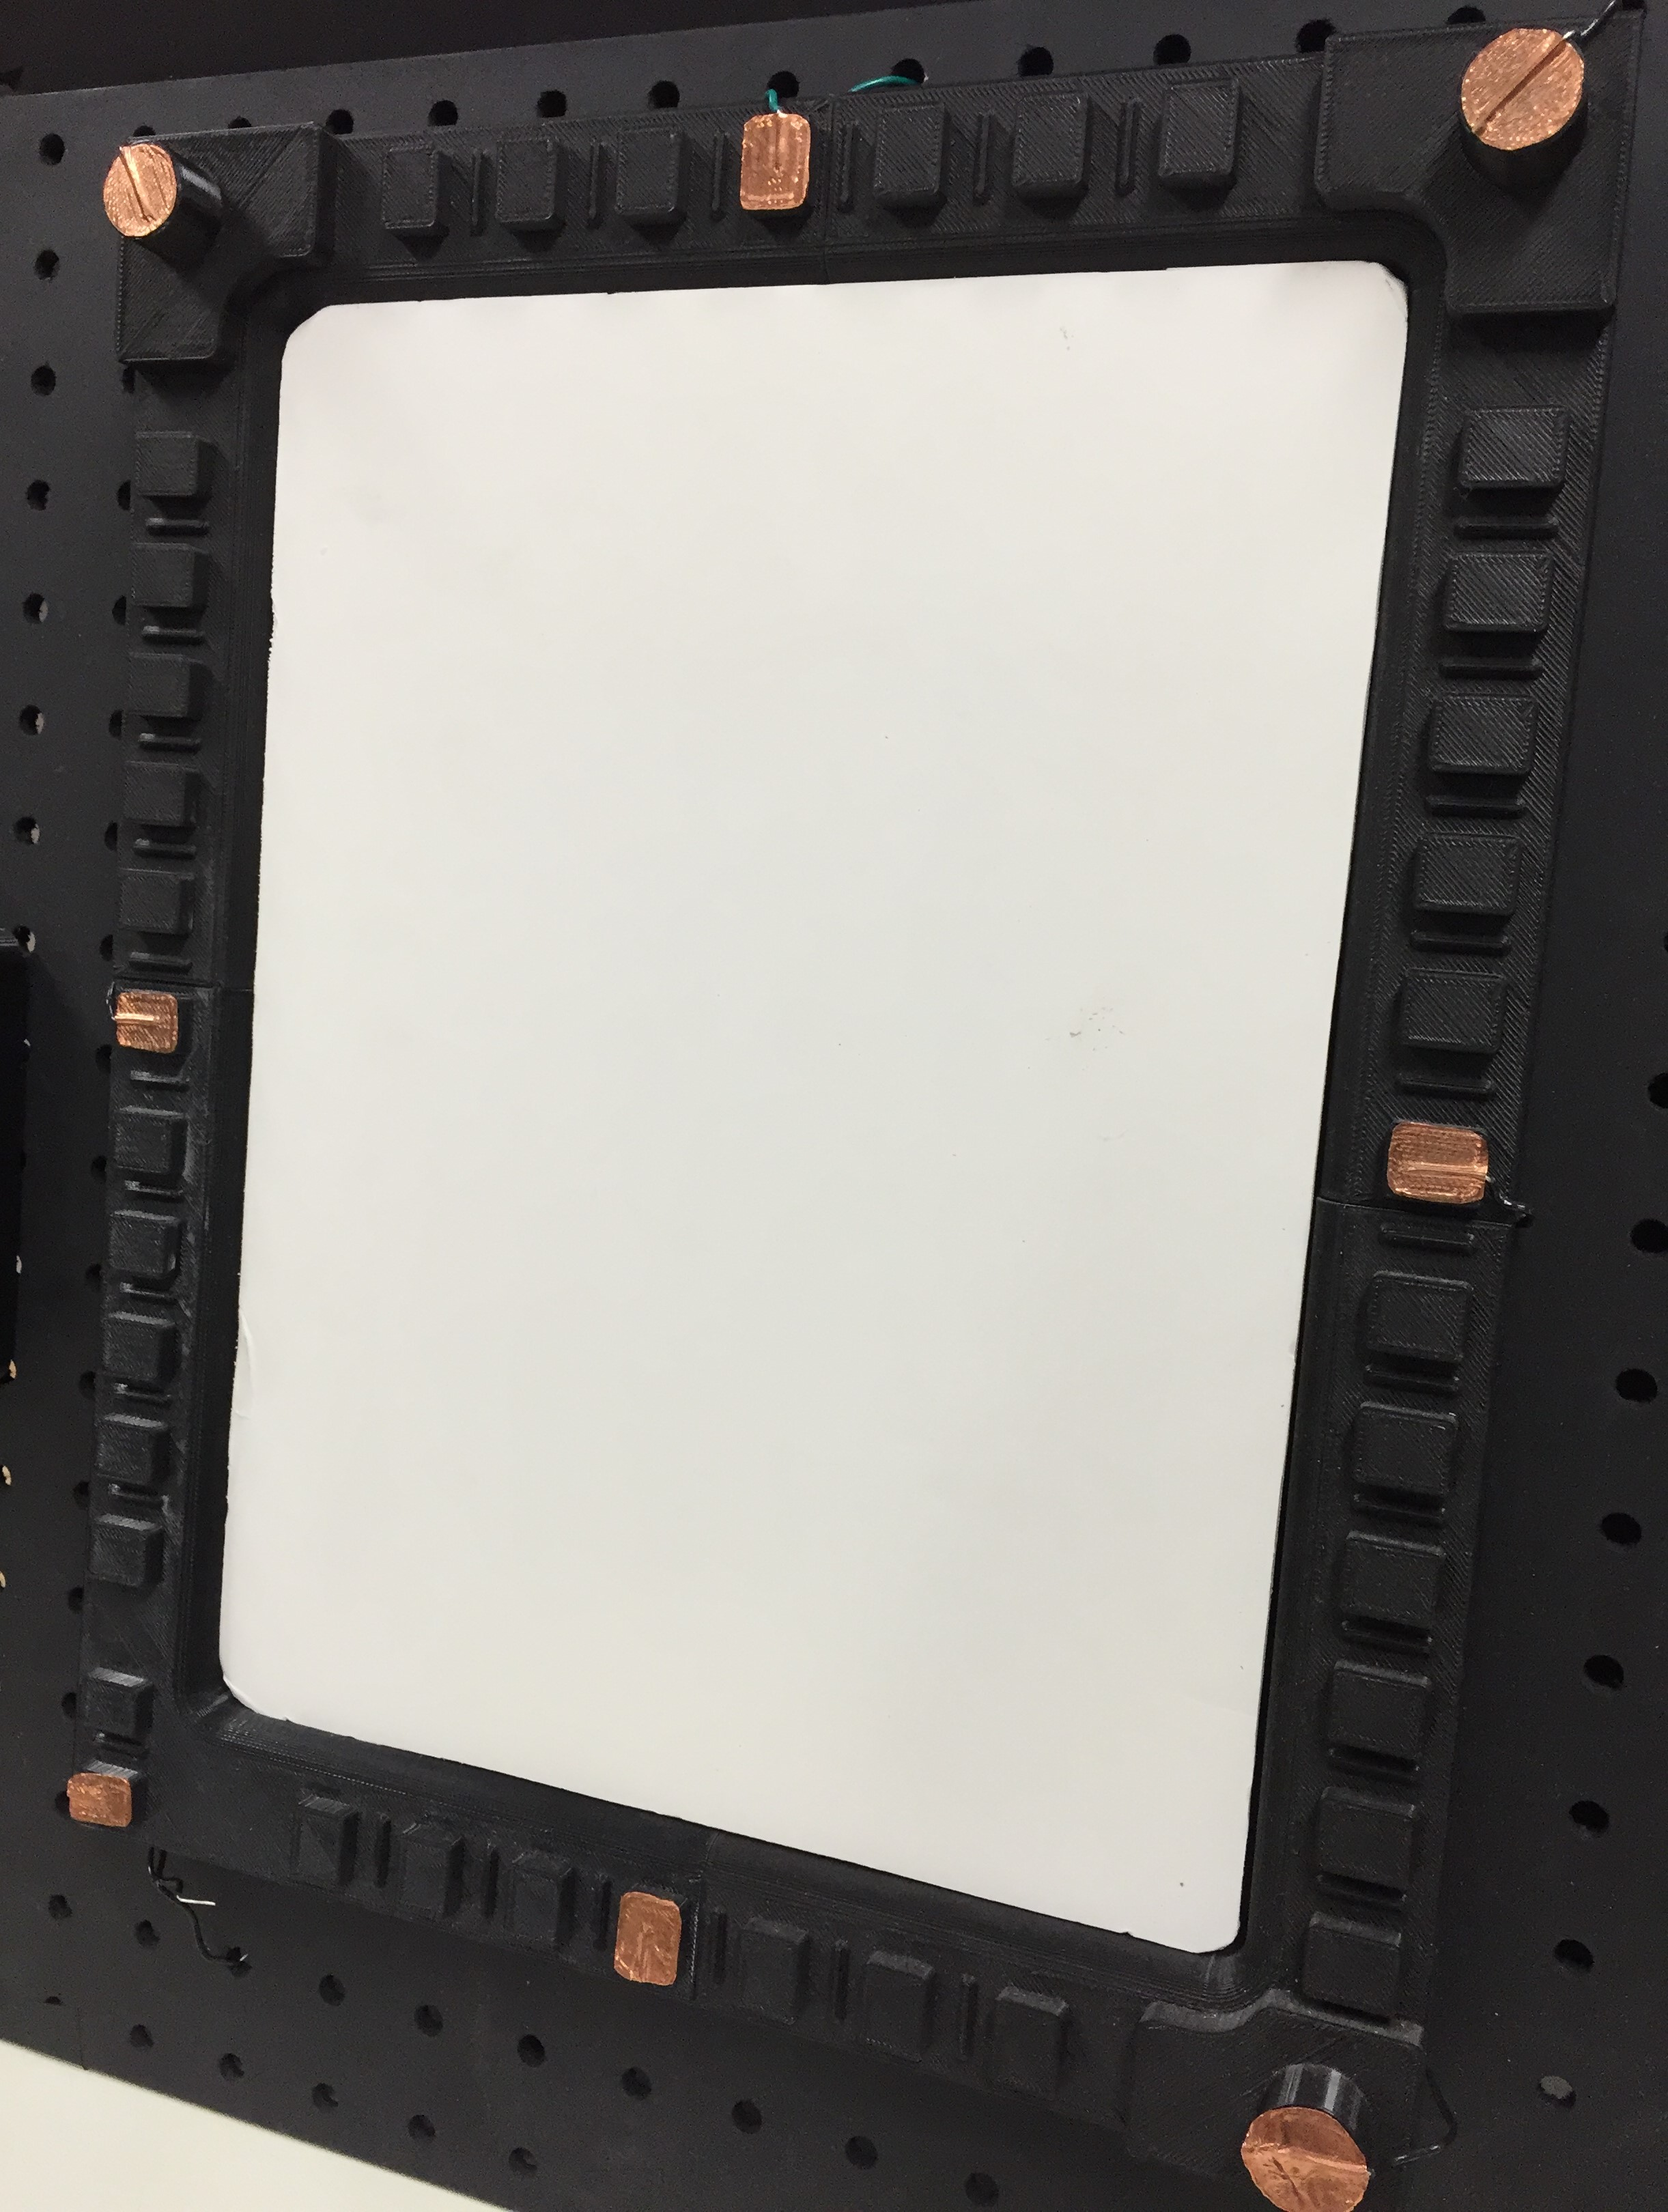
\includegraphics[width=0.5\linewidth]{copper_pads.jpg}
    \caption{The copper tape electrodes for capacitive touch sensings on the demo multifunction instrument.}
    \label{fig:copper_pads}
\end{figure}

Since touch accuracy can be important in safety-critical applications, we developed the ability to record where on the button the finger press was located using a capacitive touch sensor.
To accomplish this, a custom printed circuit board was developed that provides an electrode array of 5 rows and 5 columns over a 1-inch by 1-inch square.
This board is show in Figure \ref{fig:proto_capacitive_array}.%, where it is mounted in a 3D printed instrument.
The capacitive state of each row and column can provide a measurement of the center of the finger press on the grid created by the rows and columns.
Finger location accuracy of under 0.1-inch can be achieved with this configuration.
The location of the finger press can help provide a measure of the accuracy of the registration between the optical sensors and the real world location, as well as any bias introduced from using the VR headset and hand tracker.

\begin{figure}
    \begin{subfigure}[t]{0.32\linewidth}
    \centering
    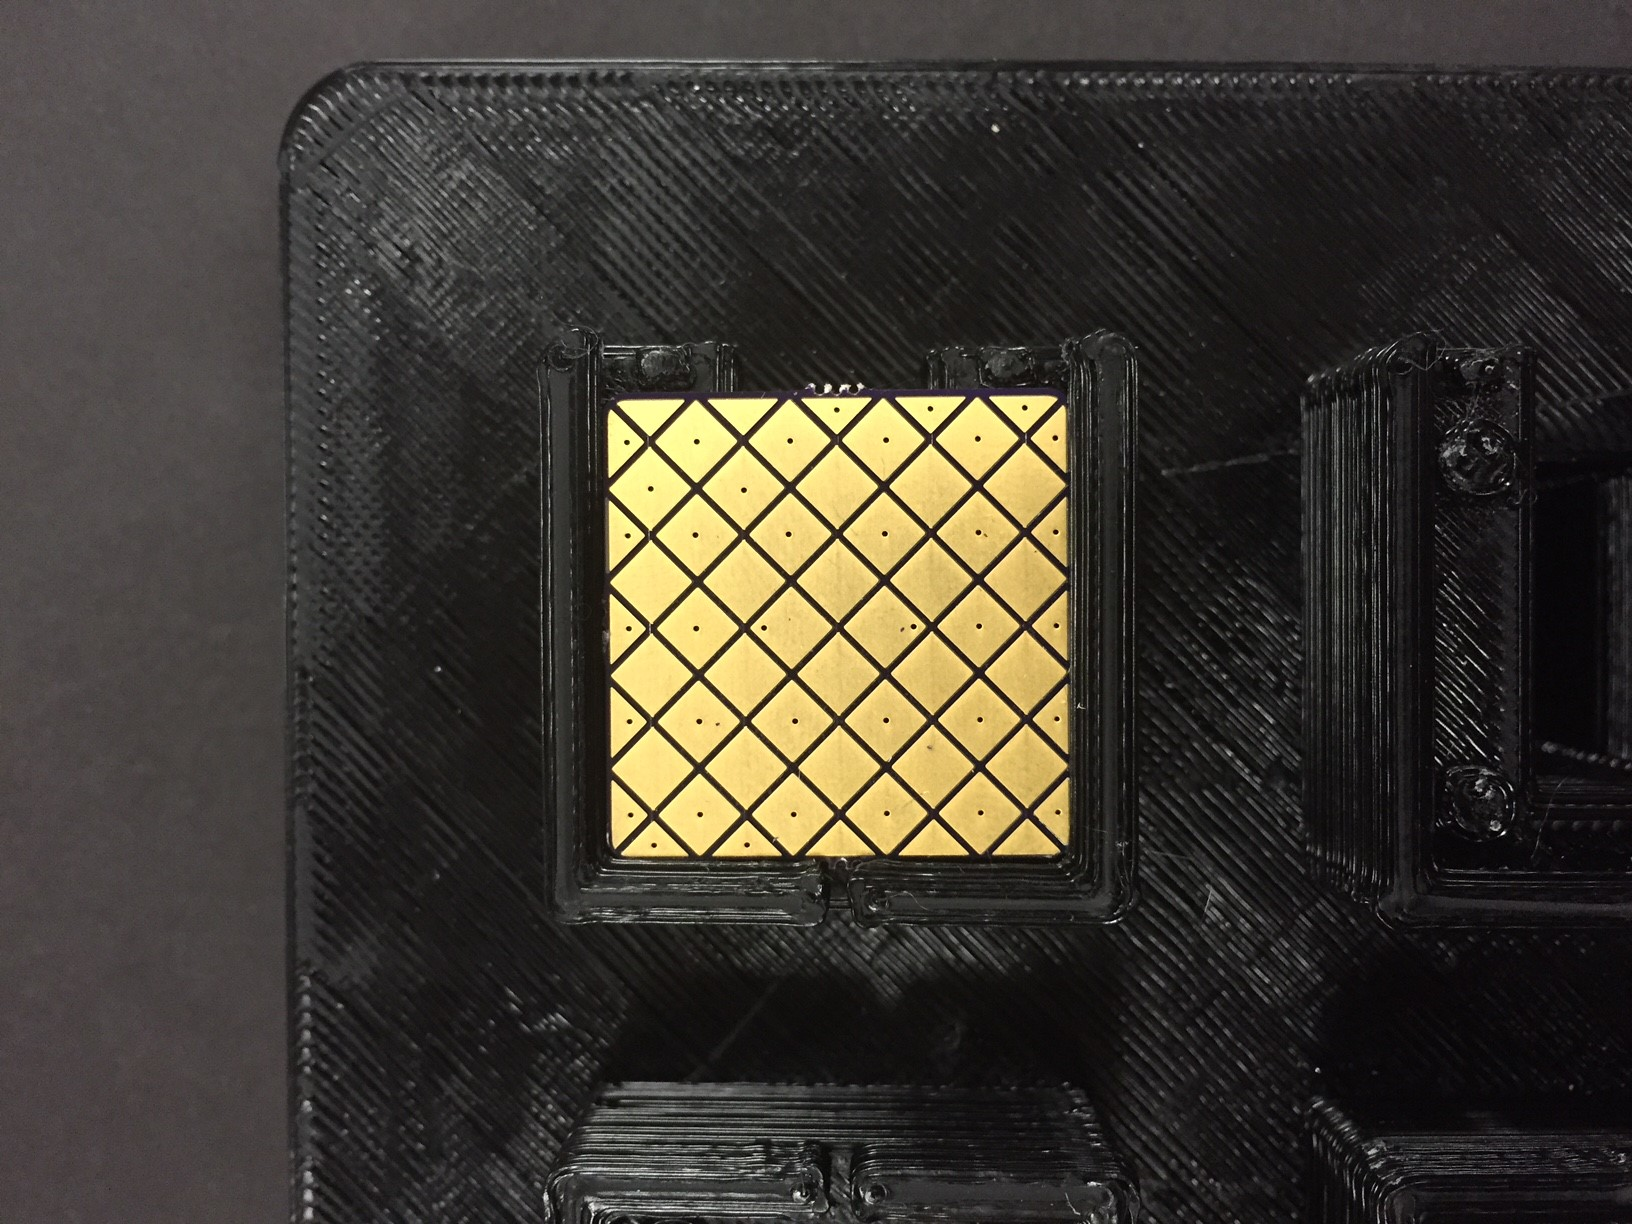
\includegraphics[width=1.5in]{pe_capacitive.jpg}
    \caption{Capactive array mounted in a 3D printed button.}
    \label{fig:proto_capacitive_array:mounted}
    \end{subfigure}
    \begin{subfigure}[t]{0.64\linewidth}
    \centering
        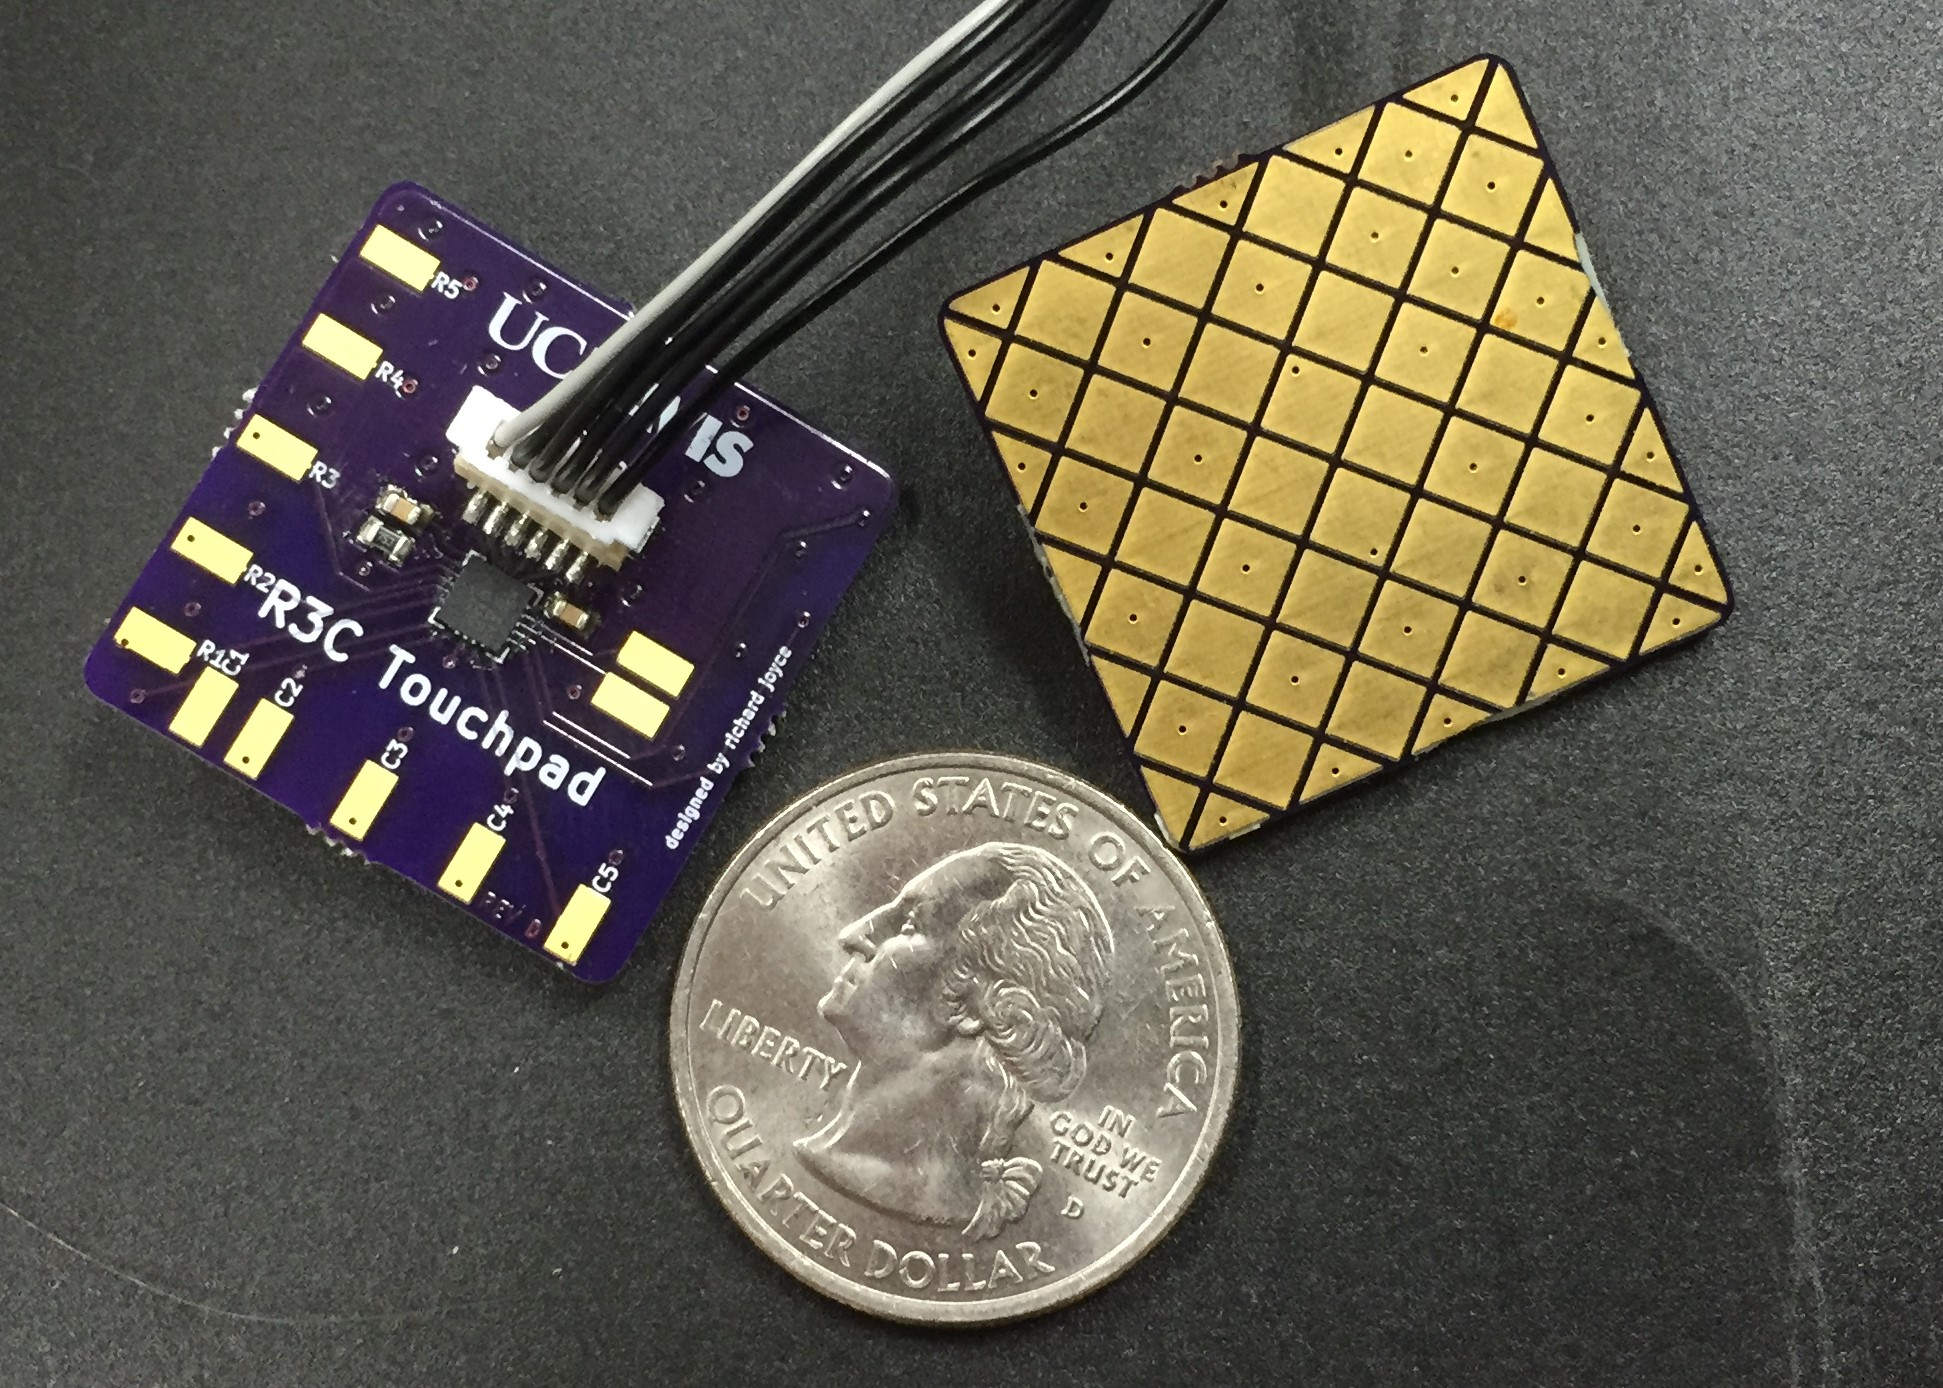
\includegraphics[width=\linewidth]{proto_cap_board.jpg}
    \caption{Bare PCB showing back and front.}
    \label{fig:proto_capacitive_array:pcb}
    \end{subfigure}
    \caption{Capacitive touch array button. Each row and column of diamond pads are connected as one electrode each and together can provide location information of where the user presses.}
    \label{fig:proto_capacitive_array}
\end{figure}

\subsubsection{Calibration}

The hand tracking of the LeapMotion provided precise and repeatable measurement of the hand positions throughout its tracking volume.
The accuracy as the hand got further away from the sensor, however, was insufficient.
Put another way, the position of the hand in the virtual world was offset from the true button position in the physical world, yet the offset was consistent between movements.
This led us to develop a calibration to provide a more accurate registration between the virtual and physical hand positions.
With the addition of the capacitive touch sensors, a calibration mechanism was made possible since it allowed for well known positions in the physical world to be translated to the virtual world.
The location of the buttons are well known from the dimensions of the physical world setup.
This means that when a finger was placed on a physical button with a capacitive sensor, the known position can be recorded along with the ``measured'' position of the hand tracker.
After collecting enough points, the calibration can correct for the measured offset and provide an accurate registration between the real and virtual worlds.
The mathematical basis for this calibration is described here.

The calibration works on the assumption that there exists a transformation matrix, $\mathbf{T}$, that can solve the following equation:
\begin{equation}
    \vec{x}_{known} = \mathbf{T}\vec{x}_{measured}
    \label{eq:proto_Tvec}
\end{equation}
The $\vec{x}_{known}$ and $\vec{x}_{measured}$ correspond to the known location of a calibration point (button) and the location measured by hand tracker, respectively.
Since we know those two vectors, it is only required to solve for the transformation matrix itself.

A simple least squares approach is used to find the coefficients of the matrix. % the registration between the virtual and physical worlds is vastly improved.
The transformation matrix is not constrained to a simple rotation (i.e.\ not assumed orthogonality or other special properties) so the solution is found by expanding and solving the general homogeneous coordinates transformation matrix.
\begin{equation}
    \begin{bmatrix}
        x_{known} \\
        y_{known} \\
        z_{known} \\
        1
    \end{bmatrix} =
    \begin{bmatrix}
        T_{11} & T_{12} & T_{13} &T_{14} \\
        T_{21} & T_{22} & T_{23} &T_{24} \\
        T_{31} & T_{32} & T_{33} &T_{34} \\
        0 & 0 & 0 & 1
    \end{bmatrix}
    \begin{bmatrix}
        x_{measured} \\
        y_{measured} \\
        z_{measured} \\
        1
    \end{bmatrix}
    \label{eq:proto_Tmat}
\end{equation}

Typical least squares approaches would attempt to find $\vec{x}_{measured}$ in Eqn.\ \ref{eq:proto_Tvec}, however we desire to find the matrix $\mathbf{T}$ itself.
It can be shown that expanding the matrix equation (Eqn.\ \ref{eq:proto_Tmat}) for the multiple calibration points (i.e.\ $\vec{x}_{known,1},\dots,\vec{x}_{known,n}$ and $\vec{x}_{measured,1},\dots,\vec{x}_{measured,n}$) and then collecting like terms will convert the problem into three different least squares problems.
They are shown here, dropping the subscripts to $k$ and $m$ for known and measured.

\begin{gather*}
    \begin{bmatrix}
        x_{k1} \\
        x_{k2} \\
        \cdots \\
        x_{kn}
    \end{bmatrix}
    =
    \mathbf{X}_M
    \begin{bmatrix}
        T_{11} \\
        T_{12} \\
        T_{13} \\
        T_{14}
    \end{bmatrix}
    ,\;\;
    \begin{bmatrix}
        y_{k1} \\
        y_{k2} \\
        \cdots \\
        y_{kn}
    \end{bmatrix}
    =
    \mathbf{X}_M
    \begin{bmatrix}
        T_{21} \\
        T_{22} \\
        T_{23} \\
        T_{24}
    \end{bmatrix}
    ,\;\;
    \begin{bmatrix}
        y_{k1} \\
        y_{k2} \\
        \cdots \\
        y_{kn}
    \end{bmatrix}
    =
    \mathbf{X}_M
    \begin{bmatrix}
        T_{31} \\
        T_{32} \\
        T_{33} \\
        T_{34}
    \end{bmatrix}
    ,\\
    \text{where}~\mathbf{X}_M =
    \begin{bmatrix}
        x_{m1} & y_{m1} & z_{m1} & 1 \\
        x_{m2} & y_{m2} & z_{m2} & 1 \\
        &\dots & & \\
        x_{mn} & y_{mn} & z_{mn} & 1
    \end{bmatrix}
\end{gather*}

Now the problem is stated with a known matrix and one unknown vector (per each of the three equations).
Once we have collected more than 4 points, it becomes an over-determined linear system, and a least squares calculation is used to find the solution.
From the solution of the three separate equations, the original $\mathbf{T}$ matrix is reconstructed.

At least 4 points are needed to solve this system, and it has been found that a calibration with small least squares residuals can be achieved with 10-20 well chosen points.
Provided no changes to the lighting or the position of components, the calibration setup can be performed once for the setup and is valid across users.

Instead of using the calibration matrix, $\mathbf{T}$, to transform all of the points in the hand, the index finger was used as the datum for the calibration.
The offset of the index finger between the measured and calibrated positions was calculated and then the entire hand was offset by this vector.
This was done as significant and unrealistic warping would occur with the virtual hand if all points were simply transformed.
This kept the relative position of each joint in the hand as reported by the LeapMotion while calibrating against the point that was most frequently used for button targeting\footnote{Subjects in all research studies were instructed to use their index finger.}.

\subsubsection{Lessons Learned}

The capacitive touch countermeasures were found to be effective, but the visual and aural countermeasures combined with more accurate registration led them to be not needed.
This hypothesis was investigated in the first research study, detailed in Chapter \ref{chap:pointing}.
We often found that a small amount of training time would improve performance.
The observations made were that new users were fixated on placing their finger where the physical feedback indicated the button was and did not adjust for misalignment with the hand tracker, while expert users learned to ignore the physical feedback and activated the hand tracker by finding the misaligned location.
Additionally, we discovered that hand pose and speed can influence the performance of the hand tracker, such that expert users can perform in the system quicker and with greater accuracy.

Not all of the input interactions with a cockpit may be appropriate or possible with just optical tracking.
Some interactions which require a fast reaction time or dynamic input (i.e.\ flight controls) may not be suitable with the current technology.
These insights also get further investigation throughout the research studies, which help quantify which tasks may be appropriate for this system.

We also initially found tracking performance degradation when the finger approached the instrument panel that was due to optical interference with the panel objects (i.e.\ it was happening only when the panel was present).
This was improved when we moved the LeapMotion to the top looking down, but the larger effect was found when looking at the raw image captured by the LeapMotion infrared cameras, discovering our black 3D printed instruments were highly reflective in infrared and showing up the same brightness as the hand.
Applying a matte paint finish improved this, and for future prototypes and configurations the reflections in infrared were monitored.
We have also found better results when covering the entire backdrop of the LeapMotion field of view with a dark matte material, as this helps provide a greater contrast between the hand and the background.

%\tinytodo{more transition}

\subsection{Third Prototype}

The third prototype was developed for the design evaluation experiment.
The motivation for the changes of the third prototype were guided more from research goals than a need for technical improvements of the system.
It is explained in more detail in Chapter \ref{chap:de_exp}, a summary is given here only to describe the technical changes to the prototype.
This premise of this experiment was to understand the utility of the R3C prototype in a design evaluation study.
For this reason, two instruments were designed, modeled, and 3D printed.
Additionally, the experiment required some subjects to use a touchscreen instead of the 3D printed instruments and hand tracker.
The touchscreen was mounted at the same location as the instruments would be (they used the same mounting plate).
The two setups (touchscreen and 3D printed) were interchangeable, and are pictured in Figure \ref{fig:proto_design_exp}.

\begin{figure}
    \centering
    \missingfigure{proto design exp jpg}
    \caption{The two configurations used in the design evaluation experiment.}
    \label{fig:proto_design_exp}
\end{figure}

With the improvements developed from the previous prototypes, the third prototype was designed to use only the hand tracker to perform input on the 3D printed cockpit instrument buttons.
The hand tracker was mounted above the instrument and pointed towards the area in front of the instrument.
For a more realistic flight simulation, the task also involved using a joystick, which was mounted to the left of subjects at desk height.
To maintain realism, the joystick was modeled in the virtual environment, and moved with the movement of the joystick in the real world.

\subsubsection{Calibration}

The calibration logic was modified for this setup to calibrate based off the position of the touchscreen.
This provided a very accurate and easy way to calibrate the hand tracker.
Instead of using the buttons on the instrument, requiring capacitive touch sensors on the buttons, the calibration was performed by switching to the touchscreen and pressing points on the screen.

One problem that was introduced with the calibration using a touchscreen was that all the points were on a single plane.
The solution to the calibration least squares problem becomes over-fit to the plane, and causes any movement perpendicular to be scaled down near to the plane, causing the hand to appear to be `stuck' to the calibration plane.
To alleviate this, an artificial point was added at 1 inch outward from the middle of the sensor datum.
The same point was added as a known and measured point, forcing the calibration matrix to fit the entire tracking volume instead of just the plane.
This technique came from previous observations which have noticed the accuracy of the sensor was better as the hand was near the tracker.
After solving this issue, the calibration became very accurate with the touchscreen as the data source for known positions.

\section{Summary}

An overview of the technical approach of the evolving Rapidly Reconfigurable Research Cockpit was presented.
The final prototype achieved many of the goals set out by the motivations and requirements.
Developments that were outside the scope of this research work and could be undertaken as future work are discussed in Chapter \ref{chap:conclusion}.
The specific configurations used in each experiment are described in detail within their respective chapter.
Some of the experiments required additional technology development that was not described here as the focus was on the R3C prototype itself.
